\section{初等函数}

See chapter 2 of  A First Course in Complex Analysis with Applicaitons. Dennis

\subsubsection{Exponential function}
\[
e^{ z }=e^{ x }\cos y+ie^{ x }\sin y
\]
\subsubsection{Arg function}

For $z\in \mathbb{C}\setminus \{ 0 \}$, $w=\mathrm{Arg}z=\arg z+2k\pi, k\in \mathbb{Z}$ has infinite many different values. $\arg z\in(-\pi,\pi]$ represents the principle value of $\mathrm{Arg}z$.

\subsubsection{Logarithm function}

$w=\mathrm{Ln}z$ is the complex number satisfying $z=e^{ w }$.
\[
w=\mathrm{Ln}z=\ln \lvert z \rvert +i\mathrm{Arg}z
\]
$\ln z=\ln \lvert z \rvert+i\arg z$ is the principle value of $\mathrm{Ln}z$.
Note that for $z_1, z_2\in \mathbb{C}\setminus \{ 0 \}$,
\[
\mathrm{Ln}(z_1z_2)=\mathrm{Ln}z_1+\mathrm{Ln}z_2,\quad \mathrm{Ln}\frac{z_1}{z_2}=\mathrm{Ln}z_1-\mathrm{Ln}z_2
\]
We use $\mathrm{Ln}$ instead of $\ln$ for the consideration of multiple values.

\paragraph{支点}

\begin{figure}[H]
\centering
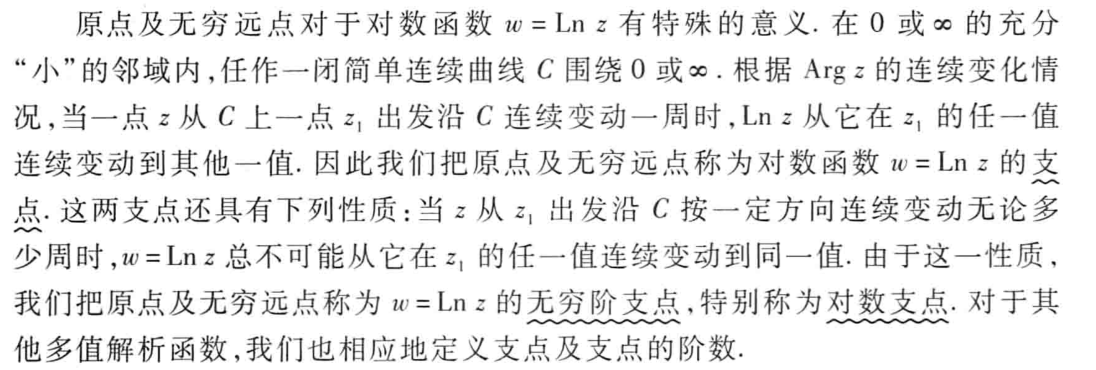
\includegraphics[width=\textwidth]{7-primary-functions-20250314.png}
% \caption{}
\label{}
\end{figure}

\subsubsection{Powers and Roots}

For $\alpha\in \mathbb{C}\setminus \{ 0 \}$, $w=z^{\alpha}=e^{ \alpha \mathrm{Ln}z }=e^{ \alpha \ln z }\cdot e^{ \alpha \cdot2k\pi i }$. $k\in \mathbb{Z}$. If $\alpha=\frac{m}{n}\in \mathbb{Q}$ then $z^{\alpha}$ is $n$ -valued. If $\alpha\in \mathbb{R}\setminus \mathbb{Q}$ or $\alpha\in \mathbb{C}\setminus \mathbb{R}$, then $z^{\alpha}$ is $\infty$ -valued.

\begin{figure}[H]
\centering
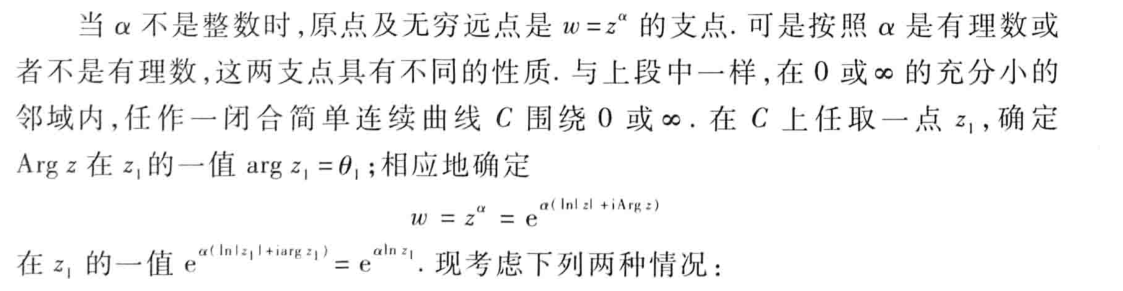
\includegraphics[width=\textwidth]{primary-functions-20250314.png}
% \caption{}
\label{}
\end{figure}

$n-1$ 阶支点:转 $n$ 圈回到最初的值。

\begin{figure}[H]
\centering
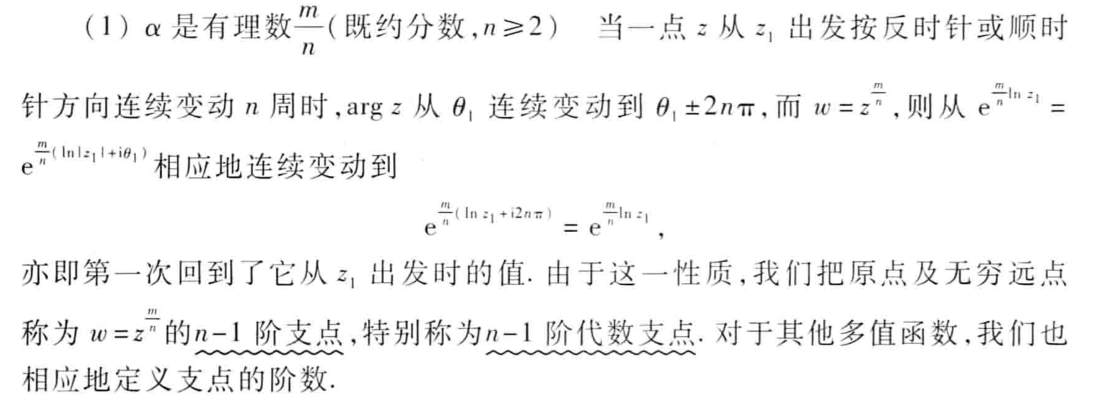
\includegraphics[width=\textwidth]{2-primary-functions-20250314.png}
% \caption{}
\label{}
\end{figure}

无穷阶支点:转不回最初的值。

\begin{figure}[H]
\centering
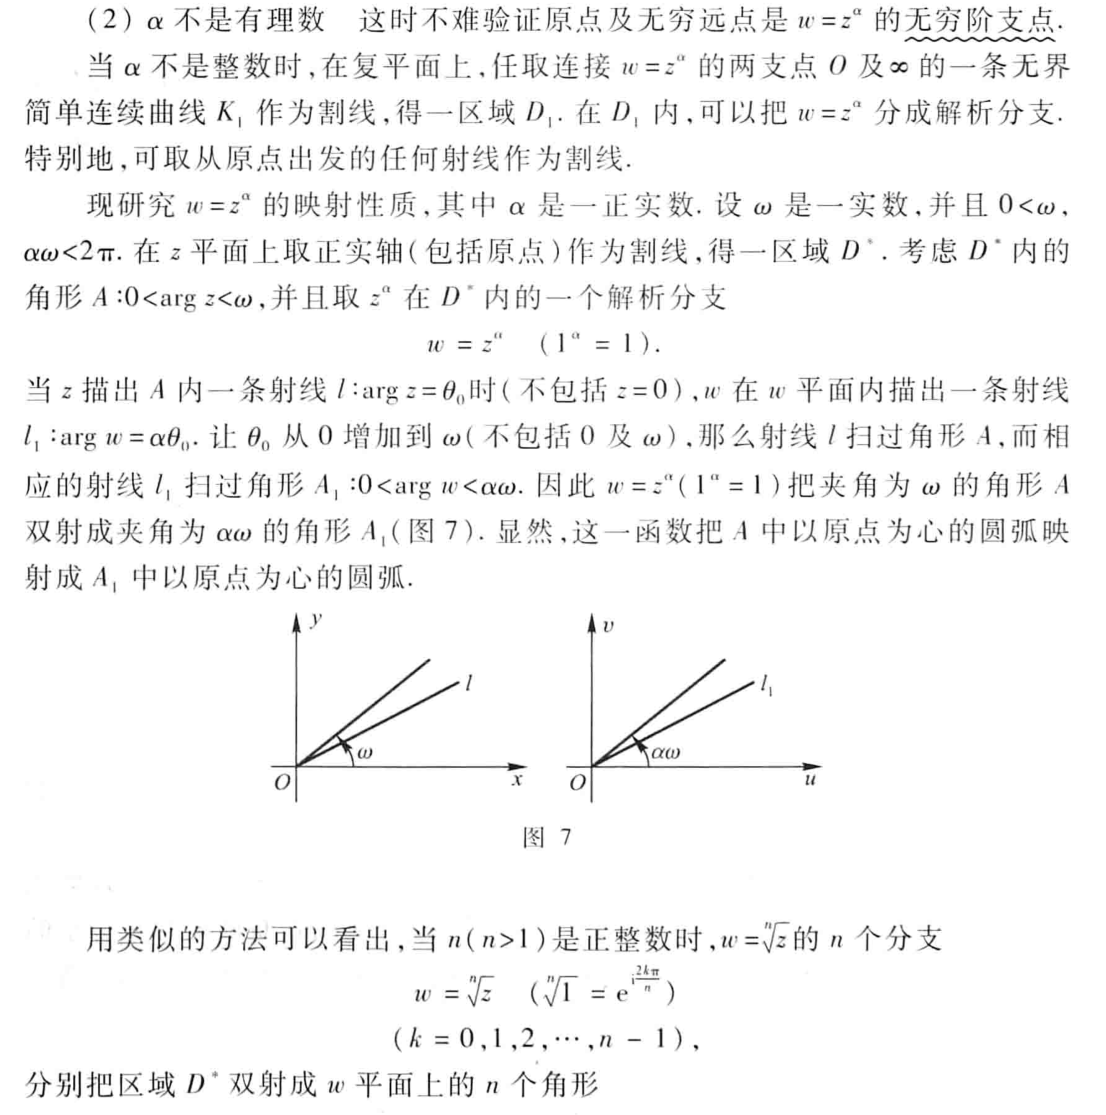
\includegraphics[width=\textwidth]{3-primary-functions-20250314.png}
% \caption{}
\label{}
\end{figure}

\begin{figure}[H]
\centering

\includegraphics[width=\textwidth]{4-primary-functions-20250314.png}
% \caption{}
\label{}
\end{figure}

\begin{figure}[H]
\centering
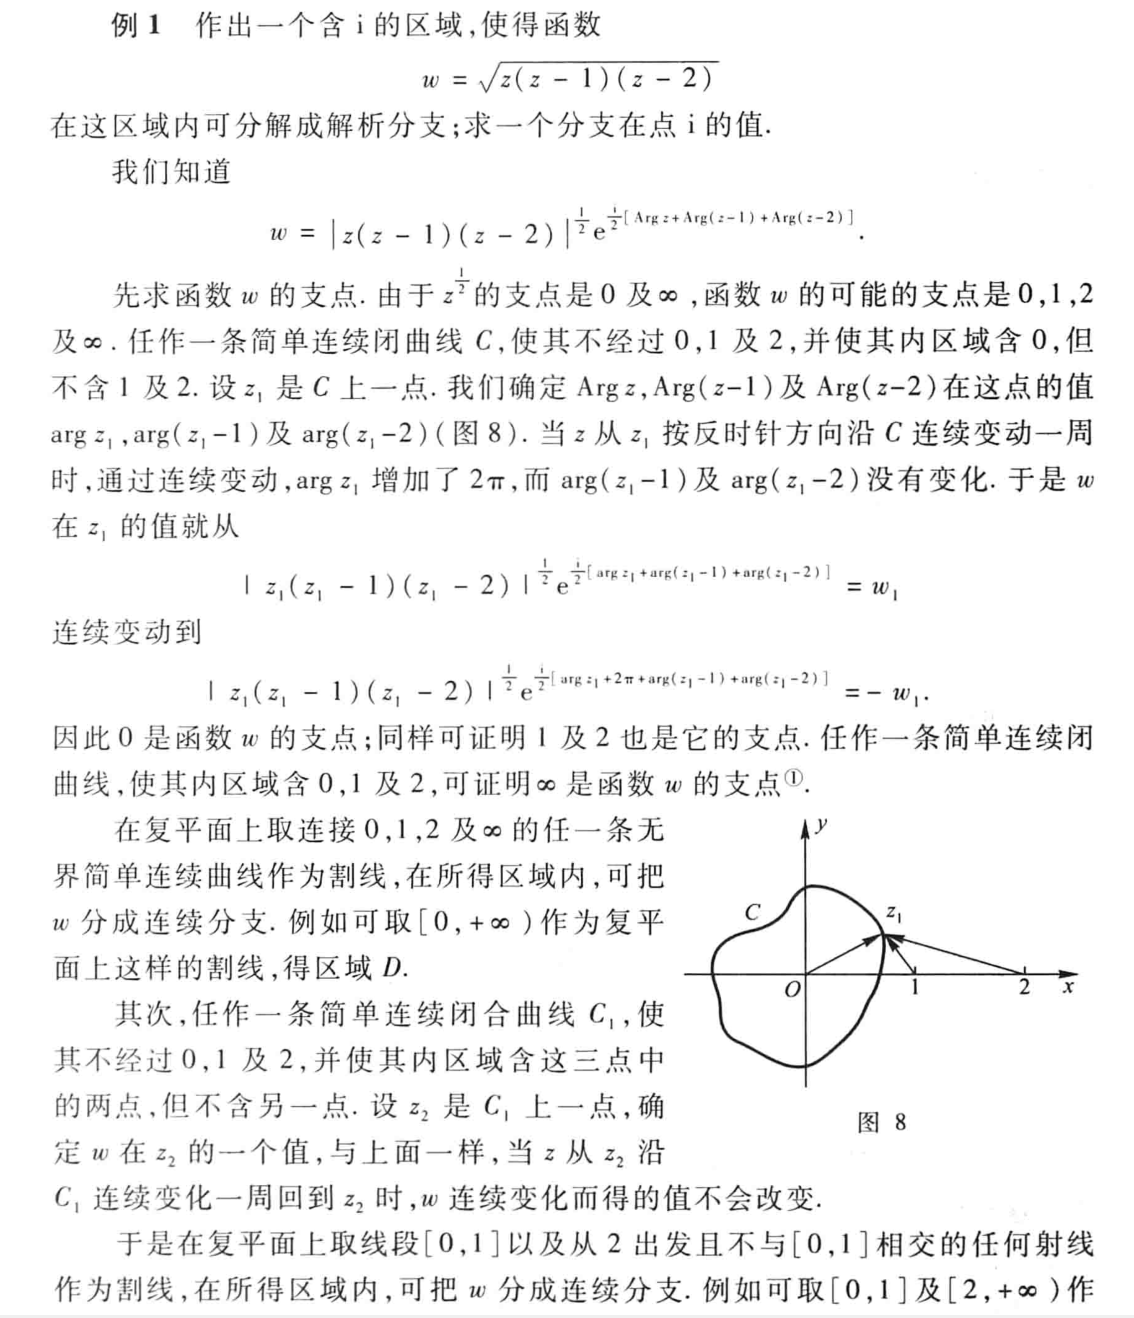
\includegraphics[width=\textwidth]{5-primary-functions-20250314.png}
% \caption{}
\label{}
\end{figure}

计算根式函数在某个给定的解析分支内的取值:

\begin{enumerate}
	\item 先计算出这个解析分支是啥,考虑极坐标
	\item 再代入给定的点到这个解析分支中
\end{enumerate}

\begin{figure}[H]
\centering
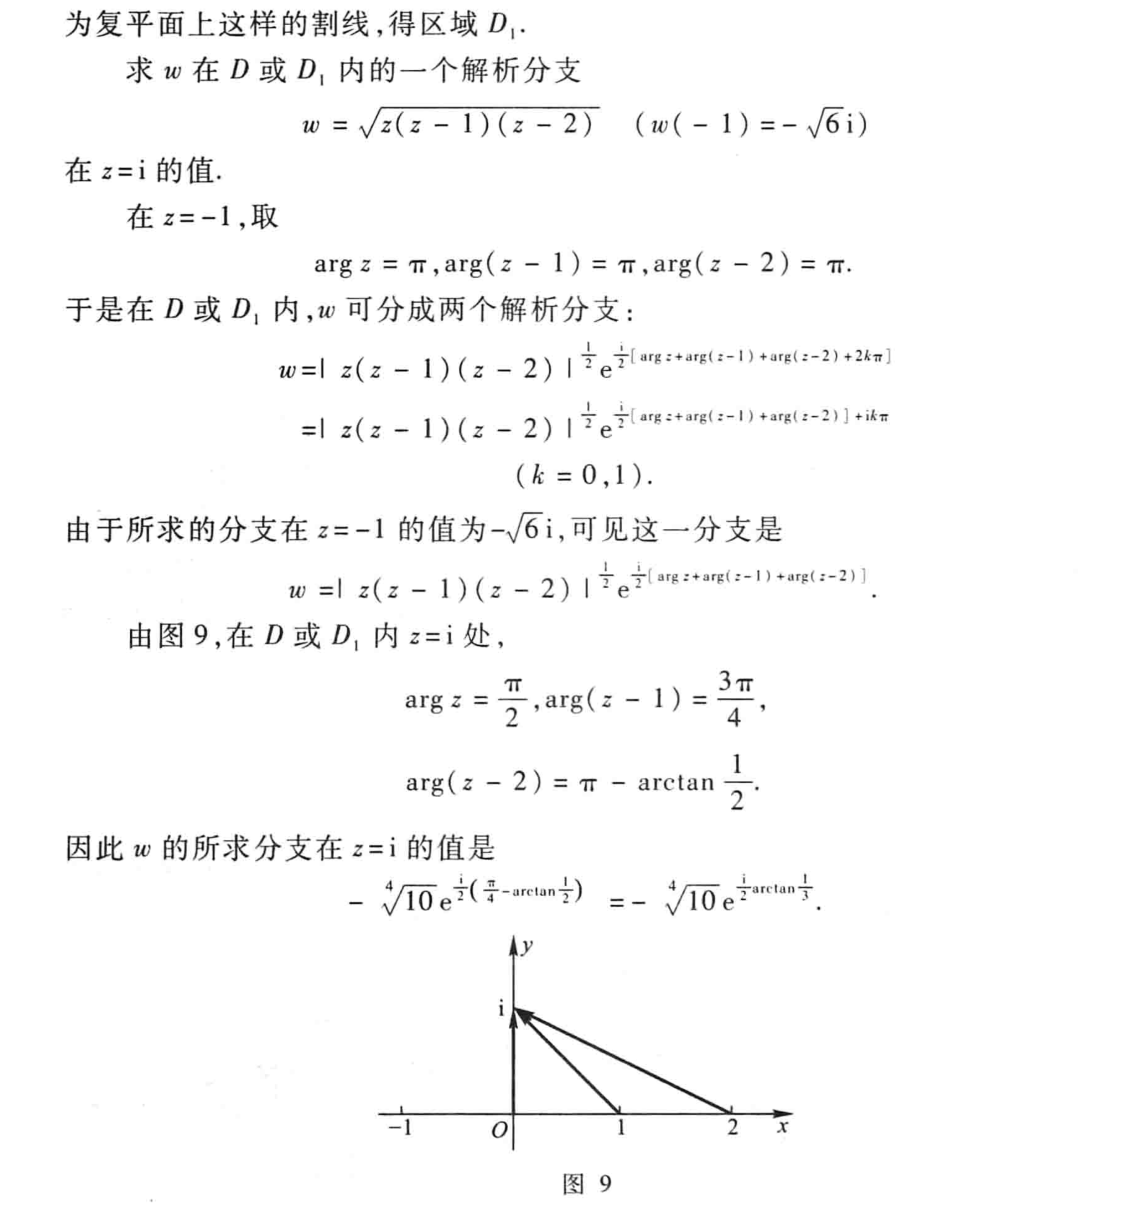
\includegraphics[width=\textwidth]{6-primary-functions-20250314.png}
% \caption{}
\label{}
\end{figure}

\begin{figure}[H]
\centering
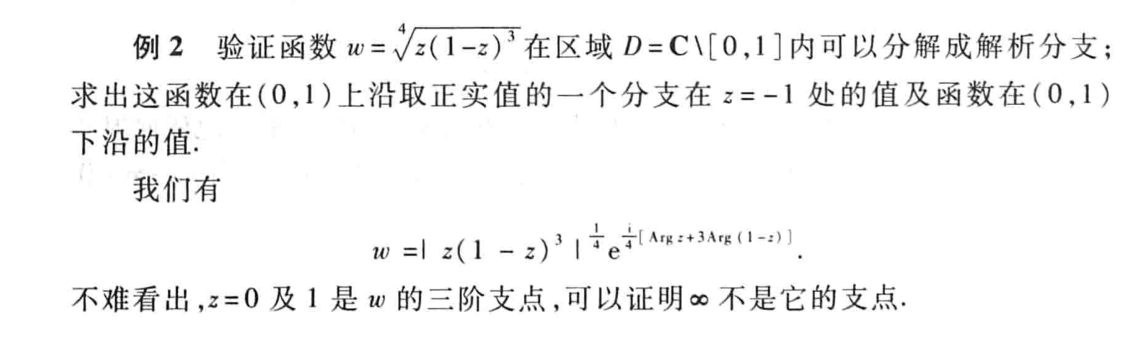
\includegraphics[width=\textwidth]{8-primary-functions-20250314.png}
% \caption{}
\label{}
\end{figure}

\begin{figure}[H]
\centering
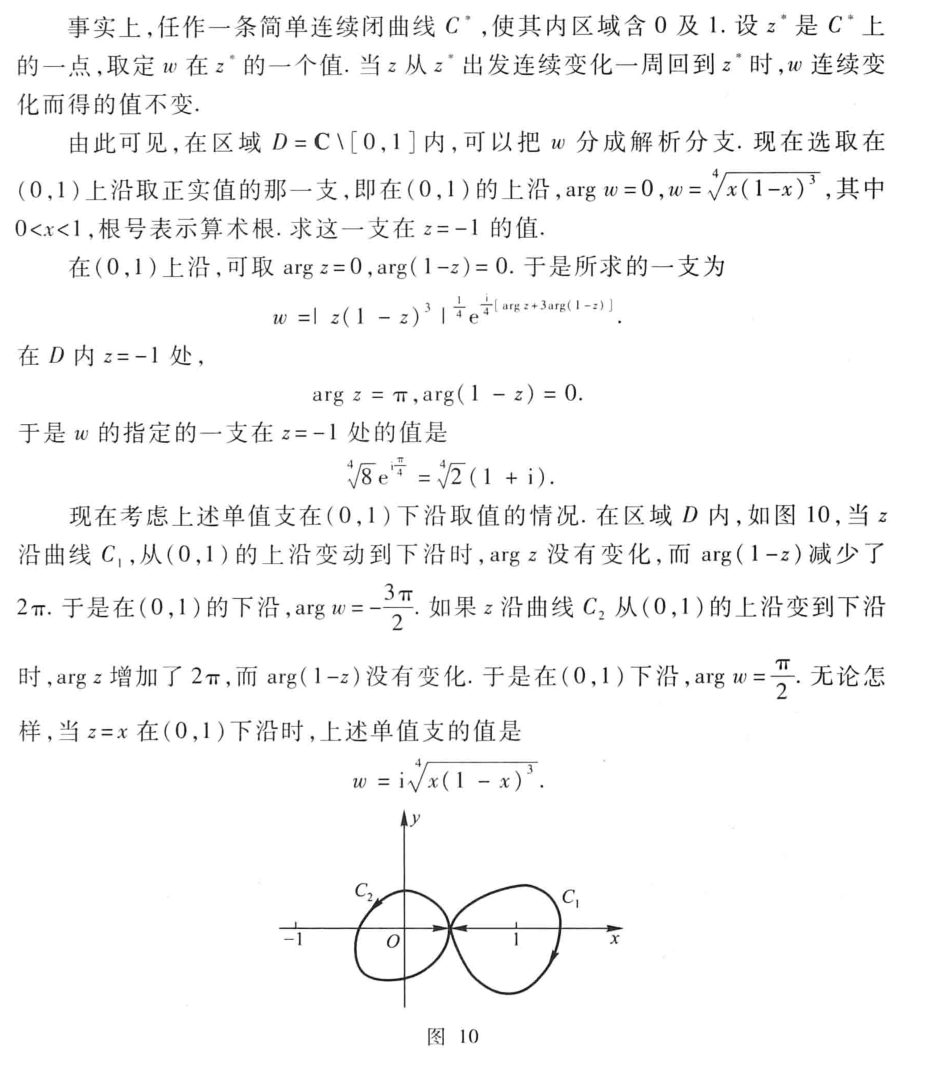
\includegraphics[width=\textwidth]{9-primary-functions-20250314.png}
% \caption{}
\label{}
\end{figure}
